
%%%%%%%%%%%%%%%%%%%%%
\subsection*{Time stratification of statistics}

Thus far we have examined how statistics vary along the genome,
but a tree sequence allows us access to another dimension: time.
Next, we examine the \emph{time} distribution of admixture signal
in the tree sequence inferred by GEVA+\tsinfer.
The Branch $f_4(A, B; C, D)$ statistic for four sample sets $A$, $B$, $C$, and $D$
is the sum of $(p_A - p_B)(p_C - p_D)$ across branches, multiplied by span and length,
where $p_X$ is the proportion of samples in sample set $X$ that inherit from that node.
A branch with a large value is expected to contribute a large amount to the Site $f_4$,
which is calculated from genotyping data
and is used to infer historical connections between populations.
To visualize the time signature, we assigned the contribution of each branch
to its terminal node,
and then summed these values across all nodes in 50 logarithmically-spaced bins by time.
We then normalised these to sum to 1 by dividing by the total Branch $f_4$ value.

The four-tuple of sample sets for the first two statistics (PUR,TSI;GWD,JPT and ASW,CEU;MSL,CHB)
are from similar regions of the world,
and show almost identical time signatures,
even though the second set of sample sets has a value of $f_4$ nearly eight times higher.
The second two statistics (IBS,GBR;FIN,JPT and TSI,CEU;FIN,CHB) are also comparable,
and also show similar signals to each other.
These curves are noisier, because the $f_4$ values are much smaller.
For all four comparisons, the largest contribution to $f_4$ comes from
ancestors living tens of thousands of generations ago.
\plr{WHAT IS THE TIME UNIT?}
This is surprising, because $f_4$ is expected to deviate from zero due to asymmetries in tree topology
during recent history (e.g., more branches ancestral to ASW and MSL than CEU and MSL).
Furthermore, we expected the different sample sets to have much more distinct time signatures.
The shared, ancient time signatures may be because nonzero $f_4$ statistics
are due to differentially sorting ancestral variation,
or inacurracies in tree sequence inference.
It is tempting but propably unwarranted to attribute the
large downward spike between 2000 and 3000 generations in the TSI,CEU;FIN,CHB comparison
to a historical connection between the ancestors of CEU and the Finnish not shared by the Tuscans
during that time period.
Making rigorous conclusions from this sort of visualization
will require substantial validation work
to understand the various sources of bias and uncertainty.


\begin{figure}
    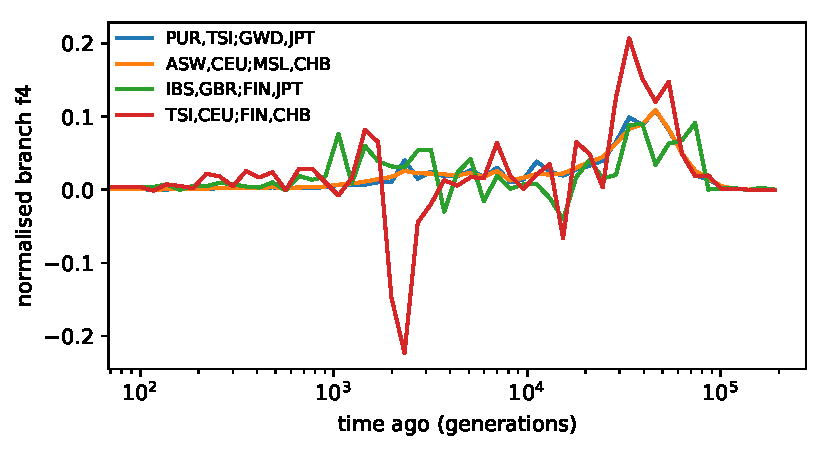
\includegraphics{{figures/1kg/tgp_geva_chr20.node.time.f4}.pdf}
    \caption{
        Time distribution of signal for four $f_4$ statistics
        in the tree sequence for chromosome 20 inferred from 1000 genomes data
        by GEVA+\tsinfer{}.
        The branch $f_4$ statistics for these four are:
        PUR,TSI;GWD,JPT: 1603,
        ASW,CEU;MSL,CHB: 12587,
        IBS,GBR;FIN,JPT: -129, and
        TSI,CEU;FIN,CHB: -96.
        Population codes are
        `PUR': Puerto Ricans from Puerto Rico;
        `TSI': Toscani in Italia;
        `GWD': Gambian in Western Divisions in the Gambia;
        `JPT': Japanese in Tokyo, Japan;
        `ASW': Americans of African Ancestry in SW USA;
        `CEU': Utah Residents (CEPH) with Northern and Western European Ancestry,
        `MSL': Mende in Sierra Leone;
        `CHB': Han Chinese in Beijing, China;
        `IBS': Iberian Population in Spain;
        `GBR': British in England and Scotland;
        and `FIN': Finnish in Finland.
        \label{fig:node_f4}
    }
\end{figure}


